\documentclass{jsarticle}
\usepackage{graphix}

\begin{document}

\section{機体}

\subsection{導入}
西田研究室では今回製作するロボカーの構成要素のうち,「制御手法」,「構成パーツ(センサなど)」,「機体設計」,の順に重要度の順位を定めた.そのため各パートの担当者と打ち合わせをしながら機体の設計を行った.設計の際にAutodesk社のCADソフト「Autodesk Inventor Professional 2018」(以下Inventor)を使用した.

\subsection{1号機}
最初にInventorで設計した1号機を図〇に示す.
機体のサイズは幅300mm,高さ120mmとなった.センサを均等に配置するために機体の形を正八角形とし,一階部分を駆動系,二階部分をセンサ系,三階部分をアームやマイコン,カメラを置くスペースとした.
この頃の設計はロボカーの制御手法や構成パーツについてあいまいな点が多く残っていたため,急な変更に対応できるようスペースを多くとるように心掛けた.

\begin{figure}[htbp]
\begin{center}
  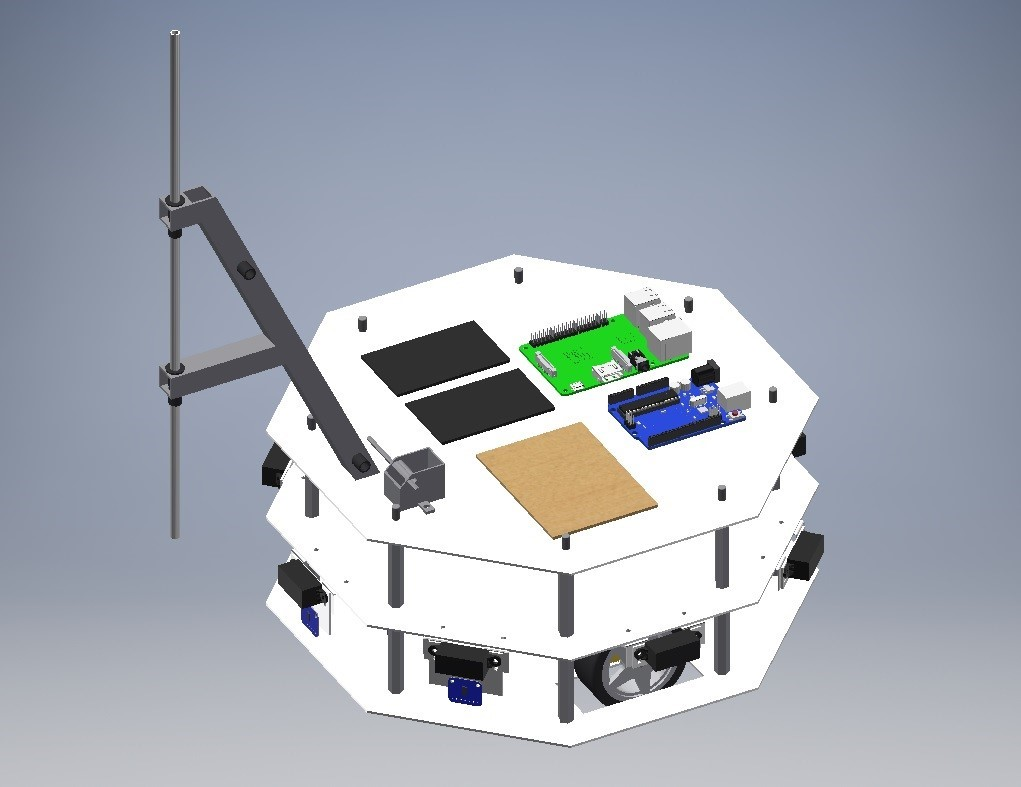
\includegraphics[width=10cm]{Documents/Final_assem.jpg}
\end{center}
\caption{1号機の概要}
\label{picture}
\end{figure}

\subsection{2号機}

\subsubsection{要求条件}
制御手法や構成パーツについての考えが固まってきた段階で,1号機の設計を元に再設計を行った.設計した2号機を図〇に示す.
再設計を行う際に各パートからの機体の要求条件を再度リストアップしてから行った.
ソフト班から求められる機体の構成
・制御のしやすい駆動系
・回転半径の縮小
・センサの測定領域の均一化
・センサの取り付け位置(高さ)
回路班から求められる機体の構成
・整備のしやすい設計
・配線への考慮
\subsubsection{改善点}
1号機では三階建てで構成していたが,一階部分には主にモーターとエンコーダしか置かれていないため,板を取り外し,モーターとエンコーダの配置を線対称から点対称へと変更した.これにより機体の幅を300mmから180mmに落とすことができた.次に,タイヤをナロータイヤへと変更した.これにより転がり抵抗の低減を図った.しかしタイヤの接地面積が極端に少なくなったため,路面状況によってはスリップする可能性があると考えられる.センサの配置は1号機と同様に正八角形の各辺に配置することとし,後方のセンサについては使用しないこととなったため取り外した.また,一階と二階(1号機での二階と三階部分)を20mmのスペーサーでつなぐことにした.これによりセンサの,路面からの高さを自由に変えられるので,ポールの下から3/4の位置にセンサの高さを調整した.

\subsubsection{反省点}
 今回,回路班からの要求である「整備のしやすい設計」と「配線への考慮」については応えることができなかった.原因としてはInventorでの設計時に回路基板の配置を考慮しておらず,さらに回路班が回路を作り始めたのが,機体が完成してからであったことが考えられる.この問題を改善するためには設計,製作手順を「制御手法の決定」「回路設計,製作」「機体の設計,製作」の順にする必要があると思われる.

\end{document}
